%%%% HRTF MEASUREMENTS %%%%
\chapter{Head-related transfer function measurements}\label{chap:A4_HRTF_Measurements}
In this appendix, we describe the measurement and data processing procedures employed in the present thesis (see \chapref{chap:05_Proposed_Models}) to capture the head-related transfer functions (HRTFs) of human subjects.
These procedures were developed and published as part of an on-going project to generate a database of HRTF and morphological measurements of humans and mannequins \citep{Sridhar2017}.
Since only a few such databases are freely available, this database was created to facilitate the development of data-driven HRTF estimation techniques, which require large datasets of measured HRTFs and morphological data.
In the original paper, the head scanning and corresponding processing procedures are also described, but we omit these details here.

\section{Introduction}\label{sec:A4_HRTF_Measurements:Introduction}
Head-related transfer functions (HRTFs) of an individual describe the idiosyncratic filtering of incident acoustic waves by the individual's morphology and are widely used in synthesizing binaural signals for spatial audio reproduction.
The most accurate way to acquire HRTFs is via acoustical measurements in an anechoic chamber \citep[chapter 2]{Xie2013}.

% We need individually measured HRTFs for our research
Many publicly available databases exist that include measured HRTFs for many human subjects and mannequins \citep[for example]{SOFAHRTFDatabasesURL}.
However, these databases are not perfect; many of the measured head-related impulse responses (HRIRs) from both the RIEC \citep{Watanabe2014,RIECHRTFDatabaseURL} and CIPIC \citep{Algazi2001} databases have undesirable pre-responses prior to the main impulses, which may make the data unreliable for use without sufficient post-processing.
Furthermore, it is not guaranteed that, for any given individual, a suitable set of HRTFs will be found in any existing database.
Consequently, in order to provide the highest-spatial-fidelity in listening tests and minimize errors in HRTFs as a source of error in the test results, individual HRTF measurements should be made for every listening test subject.

% Also, putting together a database helps the community
Since individual measurement of HRTFs is commercially infeasible, alternative techniques for estimating HRTFs have been proposed, many of which are summarized by \citet{Xie2013}.
Most techniques require morphological data that includes either measurements of specific anthropometric features \citep{Bilinski2014} or complete 3D scans of the individual's morphology \citep{Gumerov2010}.
Data-driven techniques additionally require corresponding measured HRTFs of a large number of individuals.
These HRTFs typically serve as benchmarks for validating different techniques either objectively or via subjective listening tests, and also serve as training data for data-driven techniques.
For example, a recent data-driven technique to compute HRTFs directly from head scan point clouds requires measured HRTFs and 3D head scans of many individuals as training data \citep{SridharChoueiri2017}.
Consequently, gathering new HRTF and 3D morphological scan data enables others to develop and improve such HRTF estimation techniques.

Recognizing the growing need for measured HRTF and 3D morphological data, we have begun an on-going project to measure HRTFs and 3D scans of humans and mannequins, which we compile into a publicly available database.
In \secref{sec:A4_HRTF_Measurements:Measurement_Procedure}, we present details of the measurement procedures.
In \secref{sec:A4_HRTF_Measurements:Data_Processing}, we describe the signal processing performed on the measured data.
We visualize a sample of the data in \secref{sec:A4_HRTF_Measurements:Data_Visualization} and summarize our work in \secref{sec:A4_HRTF_Measurements:Summary}.

\section{Measurement procedure}\label{sec:A4_HRTF_Measurements:Measurement_Procedure}
We conduct acoustical measurements in a $3.6 \times 2.35 \times 2.55$~m ($l \times w \times h$) anechoic chamber with 8-inch deep (equal to $1/4$ wavelength at $\sim425$~Hz) anechoic foam wedges.
In the chamber, we place a circular arc which stands vertically and is aligned to be concentric with the ``origin'' of the chamber (i.e., where the center of the subject's head is ultimately placed). 
We attach to the arc eight loudspeakers (Genelec 8030A), which are equally-spaced (in $15^\circ$ increments) between $-30^\circ$ and $75^\circ$ elevation, and we include a ninth loudspeaker mounted on a separate stand at $-57^\circ$ elevation.\footnote{Here, we use the same spherical coordinate system as that defined in \citet{AES69-2015}.}
Specifically, we align the high-frequency drivers of the loudspeakers with these elevations such that the distance from each high-frequency driver to the origin is approximately $0.76 \pm 0.005$~m.
We also place, directly below the origin, a custom-built chair that is affixed to a computer-controlled turntable (Outline ET250-3D), whose axis of rotation passes through the origin of the chamber.
The chair, which is designed to have a minimal effect on incident acoustic waves,
consists of a drum-throne seat with backrest and a thin ``headrest'' structure that provides a reference for positioning the subject's head,
in order to minimize head movements during measurements.
An image of the setup is shown in \figref{fig:HRTF_setup}.

\begin{figure}[t]
\begin{center}
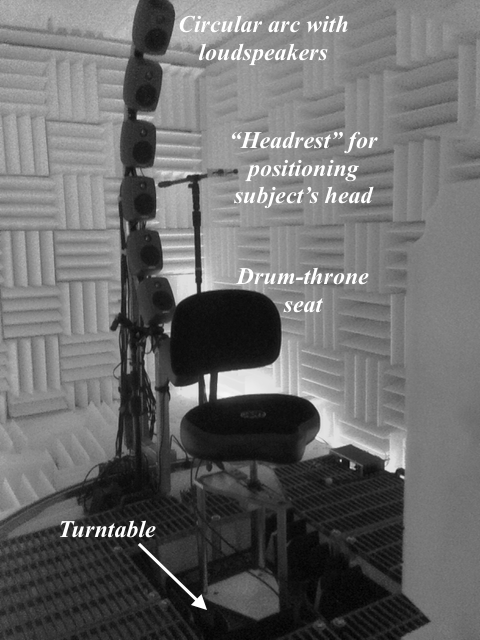
\includegraphics[width = 0.7\textwidth]{a4_HRTF_measurements/figures/HRTF_setup.png}
\caption{Setup used to make HRTF measurements.}.
\label{fig:HRTF_setup}
\end{center}
\end{figure}

Prior to making measurements, we calibrate and equalize the binaural microphones (Theoretica Applied Physics BACCH-BM Pro).
We first adjust, for each channel, the microphone gain (using a B\&K Type 4231 calibrator and DP-0978 adapter) such that a 94~dBSPL (rms) sine tone produces a $-11$~dBFS (peak) signal.
We then place the microphones at the origin of the chamber, facing the arc and parallel to the horizontal plane, in order to measure a set of nine ``reference'' impulse responses (RIRs), one for each elevation. % Joe: What about mic directivity? Rahul: Maybe we don't need to address this here. Perhaps in an auxiliary document?
For these measurements, we remove the seat cushion, backrest, and headrest, and then cover the remaining metal structure of the chair with anechoic foam wedges in order to minimize the acoustical influence of the chair-structure on the measurements.

We measure the RIRs by sending to the loudspeakers a series of partially-overlapping exponential sine sweeps \citep{Majdak2007} (generated in Plogue Bidule) and recording the resulting signals with the microphones. % Joe: Include speaker frequency responses? Rahul: I don't think this is necessary here. Maybe in an auxiliary document.
The delay between each successive sweep is 200~ms, yielding distinct impulse responses of up to 200~ms in duration.
All measurements are conducted at a sampling rate of 96~kHz and the sweep signals are generated with a nominal frequency range of 20~Hz to 48~kHz, a duration of 500~ms, and an amplitude (at 1~kHz) of 70~dBSPL (rms).
The measured signal-to-noise ratio is approximately 38.5~dB for each microphone.
The RIRs are used to equalize the transfer functions of each loudspeaker-microphone pair, as described in \secref{sec:A4_HRTF_Measurements:Data_Processing}.

For each subject, we measure binaural impulse responses (BIRs) for 648 directions: all nine loudspeaker elevations for each of 72 azimuths (equally spaced between $0^\circ$ and $355^\circ$).
We seat the subject on the chair such that the center of the subject's head coincides with the origin.
We then place the binaural microphones at the entrances to the subject's blocked ear canals and measure BIRs using the same multiple exponential sine sweeps described above.
The subject is rotated in $5^{\circ}$ increments and the sweeps are repeated until the measurements are complete.
In total, these measurements (including rotation time) takes $\sim11$ minutes.

\section{Data processing}\label{sec:A4_HRTF_Measurements:Data_Processing}
The head-related impulse responses (HRIRs) are obtained by equalizing, for each subject and for each loudspeaker-microphone pair, the measured binaural impulse responses (BIRs) by the corresponding reference impulse responses (RIRs).
We first apply a 42 ms rectangular window to all of the raw BIRs and RIRs.
We then generate inverse filters for the RIRs using frequency-dependent regularization,
such that the transfer function of the inverse filter is given by \eqnref{eq:A2_SABRE_Toolkit:EQ_Filter}, where now $H$ is the transfer function of a measured RIR.
The regularization function is defined by a set of parameters, which are defined graphically in \figref{fig:A2_SABRE_Toolkit:Farina_Regularization}, and whose default values are given by
\begin{equation*}
\begin{array}{l l l}
\beta_0 = 0, &f_{L0} = 100~\text{Hz}, &f_{H0} = 30~\text{kHz}, \\
\beta_1 = 10^{-3}, &f_{L1} = 50~\text{Hz}, &f_{H1} = 32~\text{kHz}.
\end{array}
\end{equation*}
These values were found to sufficiently limit any pre-responses in the equalized HRIRs (see \secref{sec:A4_HRTF_Measurements:Data_Visualization}), while retaining a wide usable bandwidth. 
Finally, we convolve the BIRs with these inverse filters and apply a Tukey window to generate HRIRs that have an approximate duration of 10 ms.
The BIRs, RIRs, and HRIRs are all included in the database as separate SOFA (spatially-oriented format for acoustics) files \citep{AES69-2015}.

\section{Data visualization}\label{sec:A4_HRTF_Measurements:Data_Visualization}
To verify that the our measured HRTFs are free of artifacts (e.g., pre-responses prior to the main impulses), we generate a surface plot of ITD estimated from measured HRTFs using a thresholding approach (see, for example, \citet{KatzNoisternig2014}) with a 20\% threshold.
\Figref{fig:Sample_ITD_surface} shows this surface plot for one of the subjects in our database.
This plot shows a plausible ITD surface, as it is generally smooth and free of discontinuities, suggesting that the data are free of significant artifacts, noise, or any other errors.

\begin{figure}[t]
\begin{center}
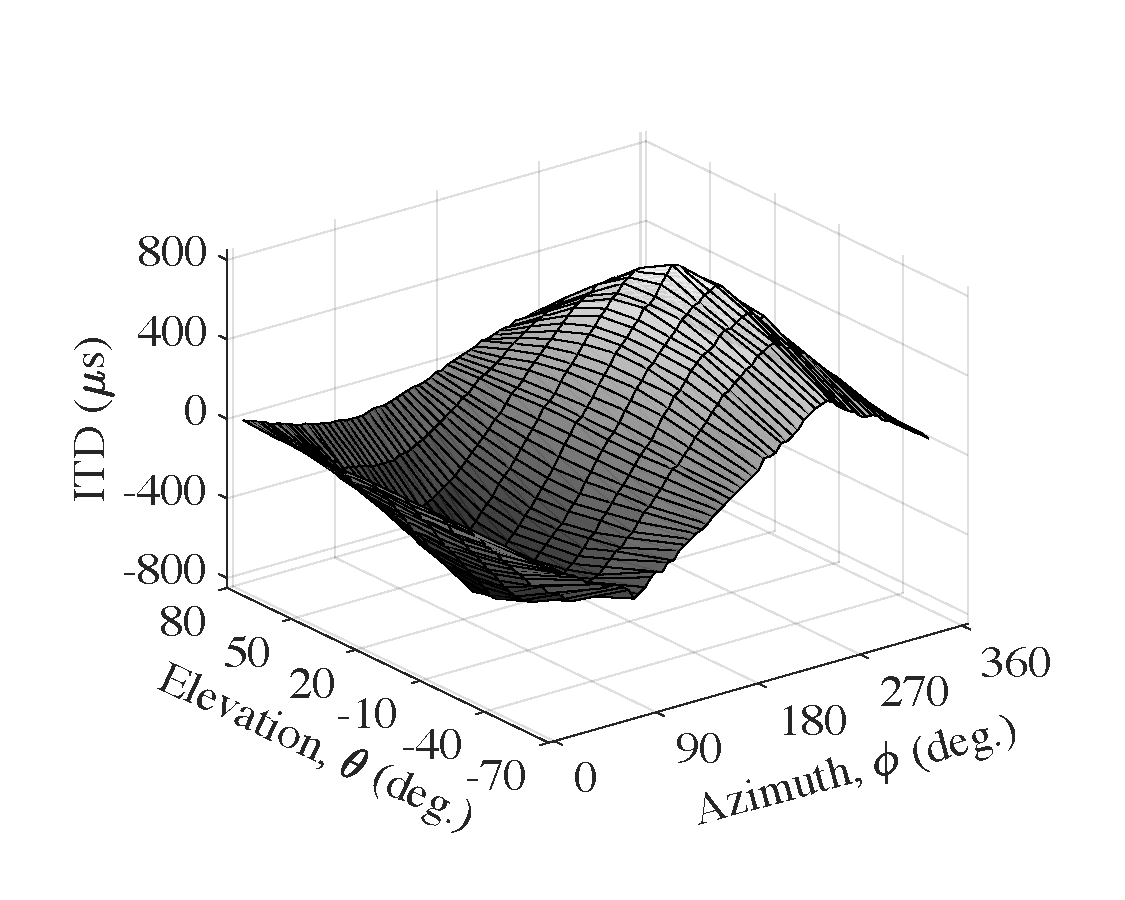
\includegraphics[width = 0.7\textwidth]{a4_HRTF_measurements/figures/Sample_ITD_surface.pdf}
\caption[Surface plot of typical interaural time differences.]{Surface plot of ITD in $\mu s$ for one of the subjects in our database.}.
\label{fig:Sample_ITD_surface}
\end{center}
\end{figure}

\section{Summary}\label{sec:A4_HRTF_Measurements:Summary}
Recently, we have begun an on-going project to measure HRTFs and 3D scans of the head and upper torso of human subjects and mannequins, and compile the data into a freely available database.
The project primarily aims to address the lack of such data.
Here, we describe details of the measurement procedures used to acquire the data and the subsequent signal processing performed.
For each subject, 648 HRTFs are measured at a distance of 0.76~m in an anechoic chamber.
We also visualize a sample of the data to illustrate that the HRTFs included in our database are free of significant artifacts and noise.
The HRTF data are stored in the standardized ``SOFA format'' (spatially-oriented format for acoustics), with separate files for BIRs, RIRs, and HRIRs (see \secref{sec:A4_HRTF_Measurements:Data_Processing}), and the database is freely available online from the 3D Audio and Applied Acoustics Laboratory at Princeton University.\citefooturl{3D3ALabHRTFDatabaseURL}

\section*{Acknowledgements}
The on-going project to generate a database of HRTF and morphological measurements has been approved by the Institutional Review Board for human subjects research at Princeton University.
The database was originally presented by \citet{Sridhar2017} at the 143\textsuperscript{rd} Convention of the Audio Engineering Society.